\begin{frame}{Sprint 2}{Overview}
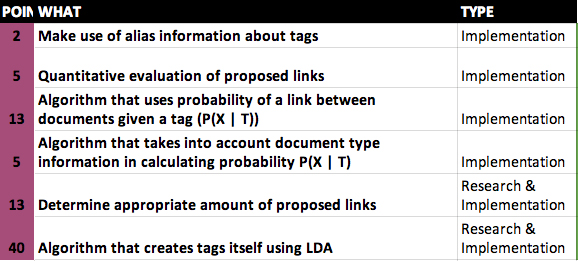
\includegraphics[width=\linewidth]{sprint.jpg}
\end{frame}

\begin{frame}{Sprint 2}{Replace aliased tags}
{\large 1. Make use of alias information about tags {\bf [2]}\\}
Each tag has a glossary, but some tags are aliases of each other and should use another tag's glossary. 
\end{frame}

\begin{frame}{Sprint 2}{Use links within the network }
{\large 'Semantic similarity' is different from heuristics used by StarFish experts.}\newline

{\large 2. Quantitative evaluation of proposed links {\bf [5]}\\}
{\bf Problem}: there are no proper links in current network\\
{\bf Solution}: network refined by expert, which will function as 'true network'
\center
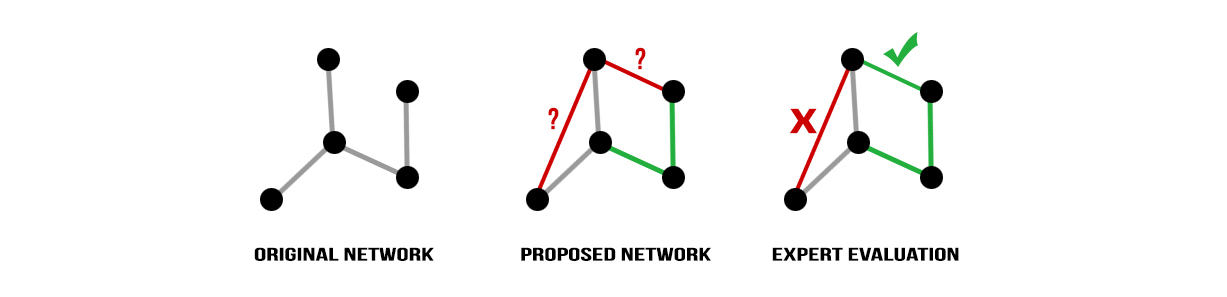
\includegraphics[width=\linewidth]{networks.jpg}
\end{frame}

\begin{frame}{Sprint 2}{Use links within the network }
{\large 3. Algorithm that uses probability of a link between documents given a
tag ($P(X \mid T)$) {\bf [13]}}\\ Calculate $P(X \mid T) = \frac{P(T \mid X)P(X)}{P(T)}$,
where X is an arbitrary link between two documents and T is a tag. \newline
\newline {\large 4. Algorithm that takes into account document type information
in calculating probability $P(X \mid T)$ {\bf[5]}}\\ Calculate $P(X | T)$ where X is
a link from one particular type to another, e.g. $X = link(Person \rightarrow
Question)$
\end{frame}

\begin{frame}{Sprint 2}{Usability}
{\large 5. Determine appropriate amount of proposed links{\bf [13]}}\\
Now the 10 best links are proposed, but sometimes less or more are really interesting.\newline \newline
{\bf Solution:} find proper threshold for Nearest Neighbor algorithm. 
\end{frame}

\begin{frame}{Sprint 2}{Dealing with missing tags}
{\large 6. Algorithm that creates tags itself using LDA {\bf[40]}}\\
{\bf Problem:} some documents have little or no tags\\
{\bf Solution:} generate 'tags' automatically using LDA, an algorithm that derivates topics from a data set.\newline \newline
Note: Difficult material, so not sure yet if we will manage to do this. 
\end{frame}

\begin{frame}{Sprint 2}{Deliverables}
\begin{itemize}
\item 'True' dataset with correct links
\item Program that can run the different algorithms and report the results (both a visual list for qualitative analysis as metrics based on a comparison with the 'true' network)
\end{itemize}
\end{frame}

\begin{frame}{Sprint 3}{Short overview}
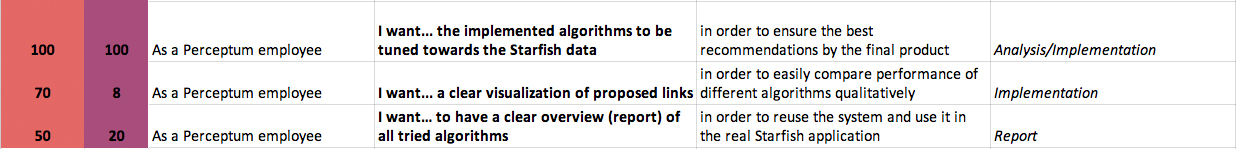
\includegraphics[width=\linewidth]{sprint2.jpg}
\begin{itemize}
\item Generating last results and analyse these together with an expert
\item Visualize last results
\item Writing of report
\end{itemize}

\end{frame}

\begin{frame}{Feedback}

{\large Thank you for listening!}\\
Are there any questions or suggestions?
\end{frame}
